%Again about two pages long
%
In this section, we will describe the model of VTSs and the properties
relevant to the biologists.

\textbf{The cell as a transport graph:} We consider a cell to be a
collection of compartments (nodes) and vesicles (edges), thus defining
a transport graph.
%
Compartments represent the large membrane-bound organelles, which are
connected by constant fluxes of small transport vesicles.
%
Every compartment or vesicle has a set of molecules associated with
it.
%
These include SNAREs and other biomolecules that regulate membrane
traffic, or that play the role of passive cargo.
%
Here we consider an abstract set of molecules and do
not explicitly associate them with particular protein varieties.\textbf{But consider them to be either of  
the two categories Q and R.}
\textbf{Molecular flows and steady state:} The total amount of each
molecular type on each compartment can increase or decrease: this is
due to gain or loss of that molecular type driven by incoming or
outgoing vesicles.
%
Each edge is thus associated with a flux of all the molecular types
carried by the corresponding vesicle.
%
We assume the cell is in a steady state where each compartments
composition does not vary over time, meaning that all incoming and
outgoing fluxes are balanced for each molecular type at each
compartment; this is the \textit{stability condition}.

\textbf{Vesicle targeting driven by molecular interactions:} The model
specification includes a description of how molecular properties
influence vesicle transport.
%
A vesicle can only contain a set of molecules that are present
on its source compartment.
%
Once a vesicle has budded out of the source, the molecules it carries
determine its properties.
%
In particular, for any given pair of a vesicle and a compartment, the
set of molecules that label the former and latter determine whether
the vesicle will fuse to that compartment.
%
Biophysically, fusion requires a direct physical interaction between
at least one molecular type on the vesicle and one molecular type on
the compartment.
%
The list of molecular pairs that can drive a fusion event is given an
a fusion pairing matrix. \textbf{For convenience, we divide Q and R SNAREs evenly 
and allow only opposite types to become a pair.}

\textbf{Molecular regulation:} The final layer of our framework
involves how the molecules are regulated.
%
We assume that for fusion to occur, the pair of molecular types
involved on the vesicle and compartment must both be in an
“active” state.
%
Whether these molecules are active or inactive depends on the
remaining molecules found on the vesicle or compartment, respectively.
%
This embodies the biological fact that other molecules can regulate the
fusion-driving molecules.
%
VTSs also require that if molecule is involved in fusion of some
vesicle and compartment, it must not be possible that the molecule 
can potentially fuse with some molecule in some other compartment.
%

We test many different versions of molecular
regulation.
%
Most generally, the activity state of a given molecule can be a
Boolean function of all the molecular types on a compartment or vesicles.
We have also tested a particularly simple regulation mechanism in which two
molecules that can pair to drive fusion inhibit one another; this is the \textit{pairing inhibition}.
%
This is motivated by the idea that pairing must generate an inactive
bi-molecular complex.

\textbf{Synthesis:} We now combine all the above ingredients.
%
Given a particular
transport graph, a particular labeling of all the compartments and edges,
a particular fusion pairing matrix, and a particular regulatory model we do
the following.
\begin{enumerate}
\item We determine which molecules are ``active" on every
compartment or vesicle.
\item or every vesicle fusing to a compartment, we
determine whether there exists an active pair (one molecule on the vesicle,
one on the compartment) which drives that fusion event.
\item For every vesicle-compartment pair where the vesicle does not fuse to the
compartment, we verify that there is no pairing of active molecules on the
vesicle and compartment that could drive their fusion.
\item We verify that every molecular type entering a compartment also leaves the compartment,
and also that every molecular type entering a set of compartments also
leaves that set.
%
This tells us that the
particular graph and molecular labeling does represent an allowed steady
state configuration of a VTS.
\end{enumerate}
%The fusion is a process where SNAREs on the vesicles target compartment is driven by the zipping together of vesicle
%and compartment SNAREs [8, 9].
%The SNAREs can be 
%Typically a Q-SNARE triple-helix is confined to one mem-
%brane surface (e.g the compartment), while an R-SNARE single helix is confined to its fusion
%partner (e.g. the vesicle). When these two types of SNAREs are in close proximity they zip
%together into a four-helix bundle, forcing the vesicle to fuse with the compartment. There are
%many types of Q-SNAREs and R-SNAREs spread between different vesicles and compart-
%ments. Across eukaryotes, there are 20 broad SNARE varieties, though individual species can
%contain higher numbers (humans have 41) [12]. Only certain Q and R-SNARE combinations
%can zip into complexes, regulating precisely which vesicles fuse with which targets. For our
%analysis, we consider a Q-SNARE triple helix as a single complex and the R-SNARE as its cog-
%nate partner. We refer to zipping as SNARE pairing.

\begin{itemize}
\item \srivas{Detailed BIO to Graph problem}
\end{itemize}


Given the above conditions, the biologists search for VTSs that are
not $k$-connected, i.e., every pair of compartments remain reachable
after dropping $k-1$ vesicles.
%
It has been observed in nature, most VTSs are 3-connected.
%
It raised the natural question what are the properties of VTSs
that are not 3-connected.
%
To study them, we have build a tool that finds VTSs that are not
$k$-connected from some $k$.

\ankit{Maximum connectivity [LGC, Least guarantee connectivity] and minimal connective [LRC (least required connectivity)] (rather than necc and suff cond) required by the graph.}

\begin{figure}
\centering
\begin{minipage}{0.50\linewidth}
  \hspace{-4ex}
\begin{tikzpicture}
\matrix [matrix of math nodes,left delimiter=(,right delimiter=),row sep=0.16cm,column sep=0.1cm] (m) {
\times & \times & \times &\times&\times&\times & \times & \times\\
\times & \times & \times&\times&\times&\times& 1 &\times \\
\times & \times & \times&\times&\times&1&\times &\times\\
\times & \times & \times&\times & 1 & \times &\times & \times\\
 \times & \times & \times & \times & \times & \times & \times & \times\\
 \times & \times & \times &\times & \times & \times & \times & \times\\
 \times & \times & \times & \times & \times & \times & \times & \times\\
 \times & \times & \times & \times & \times & \times&\times & \times\\};

\draw[dashed] ($0.5*(m-1-4.north east)+0.5*(m-1-5.north west)$) --
     ($0.5*(m-8-5.south east)+0.5*(m-8-4.south west)$);

\draw[dashed] ($0.5*(m-4-1.south west)+0.5*(m-5-1.north west)$) --
 ($0.5*(m-4-8.south east)+0.5*(m-5-8.north east)$);

\node[above=4pt of m-1-1] (top-1) {$M_1$};
\node[above=4pt of m-1-2] (top-2) {$M_2$};
\node[above=4pt of m-1-3] (top-3) {$M_3$};
\node[above=4pt of m-1-4] (top-4) {$M_4$};
\node[above=4pt of m-1-5] (top-5) {$M_5$};
\node[above=4pt of m-1-6] (top-6) {$M_6$};
\node[above=4pt of m-1-7] (top-7) {$M_7$};
\node[above=4pt of m-1-8] (top-8) {$M_8$};

\node[left=12pt of m-1-1] (left-1) {$M_1$};
\node[left=12pt of m-2-1] (left-2) {$M_2$};
\node[left=12pt of m-3-1] (left-3) {$M_3$};
\node[left=12pt of m-4-1] (left-4) {$M_4$};
\node[left=12pt of m-5-1] (left-5) {$M_5$};
\node[left=12pt of m-6-1] (left-6) {$M_6$};
\node[left=12pt of m-7-1] (left-7) {$M_7$};
\node[left=12pt of m-8-1] (left-8) {$M_8$};


\node[rectangle,above delimiter=\{] (del-top-1) at ($0.5*(top-1.south) +0.5*(top-4.south)$) {\tikz{\path (top-1.south west) rectangle (top-4.north east);}};
\node[above=10pt] at (del-top-1.north) {$Q-Snares$};
\node[rectangle,above delimiter=\{] (del-top-2) at ($0.5*(top-5.south) +0.5*(top-8.south)$) {\tikz{\path (top-4.south west) rectangle (top-6.north east);}};
\node[above=10pt] at (del-top-2.north) {$R-Snares$};

\node[rectangle,left delimiter=\{] (del-left-1) at ($0.5*(left-1.east) +0.5*(left-4.east)$) {\tikz{\path (left-1.north east) rectangle (left-4.south west);}};
\node[left=15pt,rotate=90,xshift=9mm] at (del-left-1.west) {$Q-Snares$};
\node[rectangle,left delimiter=\{] (del-left-2) at ($0.5*(left-5.east) +0.5*(left-8.east)$) {\tikz{\path (left-5.north east) rectangle (left-8.south west);}};
\node[left=15pt,rotate=90,xshift=9mm] at (del-left-2.west) {$R-Snares$};

\begin{pgfonlayer}{myback}

\foreach \element in {m-1-7,m-3-8,m-5-1,m-5-2,m-5-3,m-5-4,m-6-1,m-6-2,m-6-3,m-6-4,m-7-1,m-7-2,m-7-3,m-7-4,m-8-1,m-8-2,m-8-3,m-8-4}{
\highlight[pink]{\element}{\element}
}
\foreach \element in {m-2-7,m-3-6,m-4-5}{
\fhighlight[blue!10]{\element}{\element}
}
\end{pgfonlayer}

\end{tikzpicture}  
\end{minipage}
\begin{minipage}{0.45\linewidth}

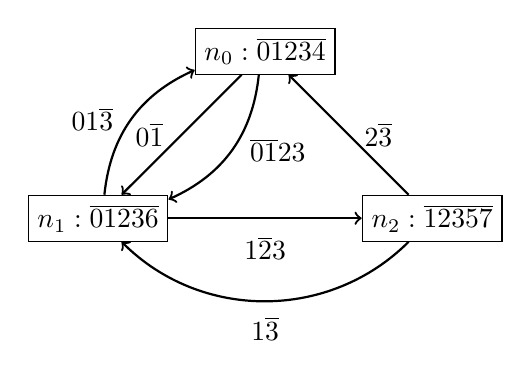
\begin{tikzpicture}[node distance = 30mm]
  \node[draw] (n0) {$n_0:\overline{01234}$};
  \node[draw,below left of=n0] (n1) {$n_1:\overline{01236}$};
  \node[draw,below right of=n0] (n2) {$n_2:\overline{12357}$};

  \draw[->,thick] (n0) -- node[left=1mm]  {$0\overline{1}$} (n1);
  \draw [->,thick] (n0) to [bend right=-30] node[right=1mm]  {$\overline{01}23$} (n1);
  \draw [->,thick] (n1) to [bend right=-30] node[left=1mm]  {$01\overline{3}$} (n0);

  \draw [->,thick] (n1) -- node[below=1mm]  {$1\overline{2}3$} (n2);
  \draw [->,thick] (n2) to [bend right=-45] node[below=2pt]  {$1\overline{3}$} (n1);

  \draw [->,thick] (n2) -- node[right=2pt]  {$2\overline{3}$} (n0);

\end{tikzpicture}
\end{minipage}

\caption{Pairing matrix} \label{fig:M1}
\end{figure}

%%% Local Variables:
%%% mode: latex
%%% TeX-master: "main"
%%% End:


\begin{example}
%
In figure~\ref{fig:M1}, we present a VTS that has 3
compartments and 8 molecules, and corresponding pairing matrix that
describes the fusion dependency.
%
Molecules are numbered 0-7.
%
In the VTS, labels consists of sting of molecule ids and overline
over an id indicates that the molecule is active.
%
This VTS is an example of version where every present molecule on
the node is active and activity of the molecules on the
edges are controlled by presence of the other molecules.
%
On the right side of the figure, we present pairing matrix.
%
An entry 1 represents pairing between molecules and
entry $\times$ represents no pairing.
% rectangles colored $\times$ one represents don't cares.
%
Everywhere in the graph the flux is maintained, i.e.,
every molecule is coming back to it's source node in a cycle.
%
The graph follows the fusion rules as discussed earlier and
is a 3-connected graph.
\ashu{R Q molecule types are not discussed anywhere.}
\end{example}

%--------------------- DO NOT ERASE BELOW THIS LINE --------------------------

%%% Local Variables:
%%% mode: latex
%%% TeX-master: "main"
%%% End:
